\documentclass{article}
\usepackage[left=3cm,right=3cm,top=2.5cm,bottom=2cm]{geometry} % page settings
\usepackage{amsmath} % provides many mathematical environments & tools
\usepackage{amssymb}
\usepackage{amsfonts}
\usepackage[spanish]{babel}



\usepackage{multirow}

\usepackage{algorithm}
\usepackage{algpseudocode}
\usepackage{pifont}

\usepackage[utf8]{inputenc}
\setlength{\parindent}{0mm}

\usepackage[parfill]{parskip}

% Para el código
\usepackage{listings}
\usepackage{xcolor}
\definecolor{gray}{rgb}{0.5,0.5,0.5}
\newcommand{\n}[1]{{\color{gray}#1}}
\lstset{numbers=left,numberstyle=\small\color{gray}}

% Entorno para estilo de ejercicios
\setlength{\parindent}{0pt}

\usepackage{color}   %May be necessary if you want to color links
\usepackage{hyperref}
\hypersetup{
    colorlinks=true, %set true if you want colored links
    linktoc=all,     %set to all if you want both sections and subsections linked
    linkcolor=blue,  %choose some color if you want links to stand out
}

\usepackage{graphicx}
\usepackage{subfig}

\begin{document}

\title{%
  \huge Análisis de la eficiencia de algoritmos \\[5mm]
  \Large Algorítmica\\
  \normalsize Doble Grado en Ingeniería Informática y Matemáticas\\[5cm]
}
\author{Yábir García Benchakhtir \\ yabirgb@correo.ugr.es \\[10cm]}

\date{\today}
\maketitle

\newpage
\tableofcontents
\newpage

\section{Análisis de los algoritmos}

\section{Cálculo de la eficiencia empírica}

\subsection{Procedimiento}

Para el cálculo de la eficiencia empírica se ha automatizado el
proceso. Para ellos se han hecho 2 scripts de bash y un archivo
makefile para realizar las siguientes tareas:

\begin{itemize}
\item Crear archivos ejecutables para todos los algoritmos programados
  en \textit{C++} con distintas opciones de optimización a saber
  \textit{O1}, \textit{O2} y \textit{O3}.
\item Ejecutar los distintos tests para los intervalos programados y
  almacenar los resultados en archivos de datos.
\item Crear las respectivas gráficas para cada tabla de datos obtenida usando la herramienta gnuplot.
\end{itemize}

Para los algoritmos de medición se ha elegido un rango de datos común
en el intervalo [1000, 25000] de manera que se toman 25 medidas
haciendo incrementos de 1000 en 1000 para tomar las medidas.

$$D = \{x \in [1000, 25000]: x = 1000k, k \in \mathbb{N}\}$$

Junto a este documento se encuentran las gráficas creadas y los datos
que proporciona el programa \textit{gnuplot} sobre las mediciones.

A la hora de hacer un ajuste de mínimos cuadrados se han usado las
siguientes funciones de ajuste:

\begin{table}[H]
  \centering
  \begin{tabular}{|c|c|}
    \hline
    Complejidad (\textit{Big O}) & Función de ajuste \\ \hline
    $O(n^2)$ & $f(x) = ax^2 + bx + c$ \\ \hline
    $O(n^3)$ & $f(x) = ax^3 + bx^2 + cx + d$ \\ \hline
    $O(nlog(n))$ & $f(x) = a\cdot log(x+b) + c$ \\ \hline
    $O(2^n)$ & $f(x) = a2^x$ \\ \hline


  \end{tabular}
  \caption{Funciones de ajuste}
\end{table}

\subsection{Condiciones de las mediciones}

Para llevar a cabo las mediciones se ha utilizado un ordenador con las
siguientes características:

\begin{itemize}
\item CPU: Intel Pentium G3258 (2) @ 3.200GHz
\item Memoria RAM: 7876MiB
\item Kernel:4.13.0-36-generic
\item OS: Linux Mint 18.3 Sylvia x86\_64
\end{itemize}

A la hora de realizar los tests se ha tenido la precaución de
minimizar el uso de \textit{CPU} para no interferir en las mediciones.

\section{Resultados obtenidos}

En esta sección de la practica me concentro en mostrar los resultados
obtenidos tras haber completado el proceso de pruebas de los distintos
algoritmos. En este caso muestro los datos con una eficiencia al
compilar \textit{O0}.

\subsection{Algoritmo de ordenación Burbuja}


\begin{figure}[H]%
    \centering
    \subfloat[Nube de puntos]{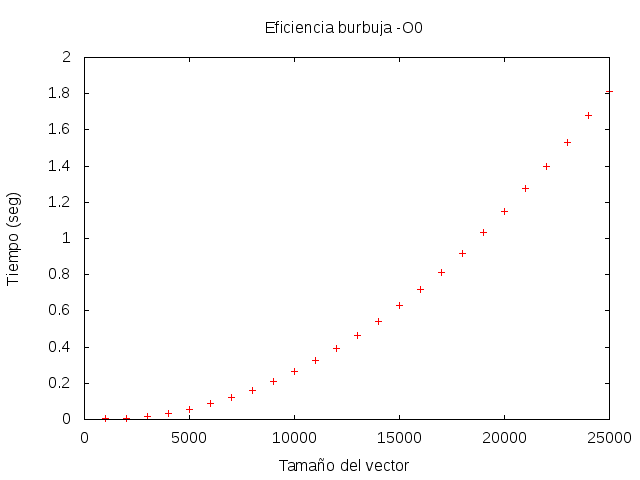
\includegraphics[width=0.5\textwidth]{../plots/burbuja_O0_points.png}}%
    \subfloat[Función continua]{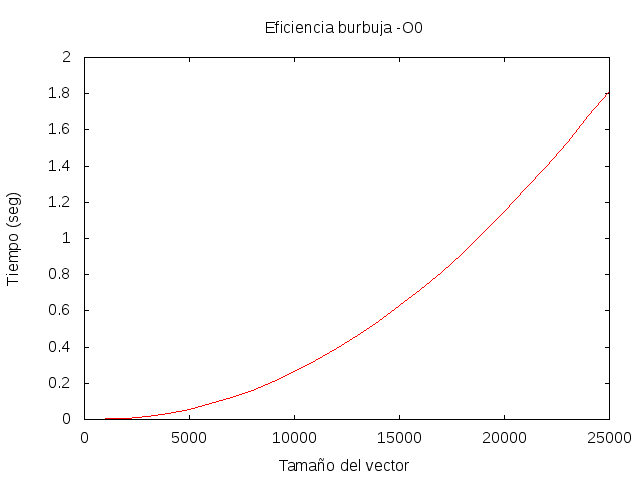
\includegraphics[width=0.5\textwidth]{../plots/burbuja_O0_lines.png}}%
    \caption{Resultados experimentales representados mediante una nube de puntos y la linea que los une}%
    \centering
    \subfloat{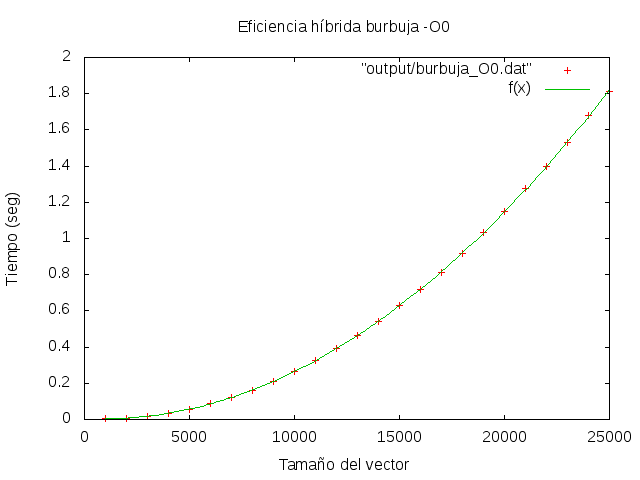
\includegraphics[width=0.6\textwidth]{../plots/burbuja_O0_fit.png}}%
    \caption{Ajuste para: ordenación usando el algoritmo de burbuja}%
\end{figure}

\begin{verbatim}
Final set of parameters            Asymptotic Standard Error
=======================            ==========================

a               = 3.11154e-09      +/- 1.128e-11    (0.3624%)
b               = -5.17483e-06     +/- 3.02e-07     (5.837%)
c               = 0.00563209       +/- 0.001704     (30.26%)


\end{verbatim}

\subsection{Algoritmo de ordenación por insercción}



\begin{figure}[H]%
    \centering
    \subfloat[Nube de puntos]{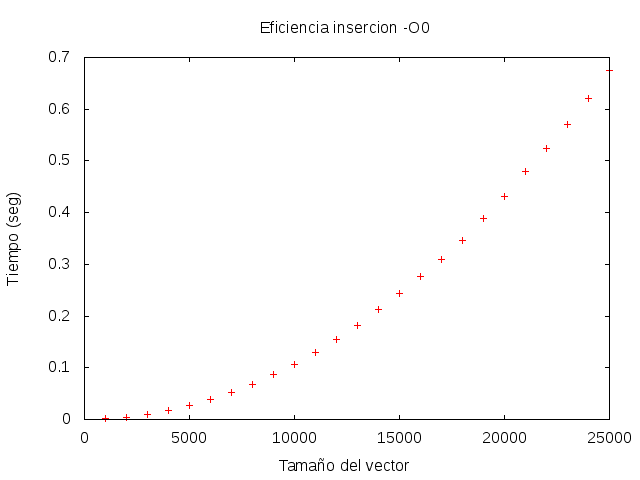
\includegraphics[width=0.5\textwidth]{../plots/insercion_O0_points.png}}%
    \subfloat[Función continua]{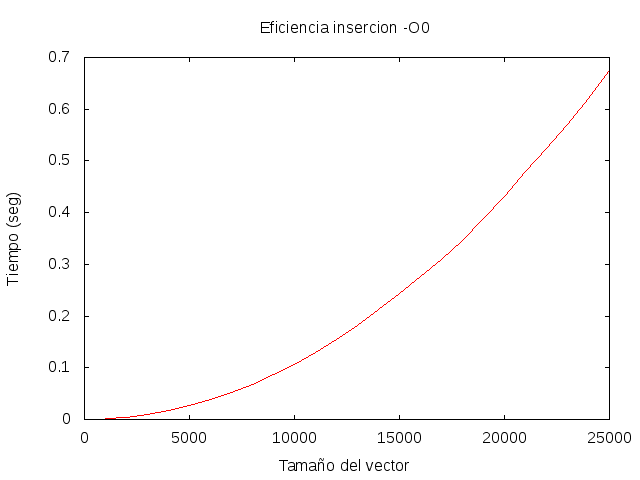
\includegraphics[width=0.5\textwidth]{../plots/insercion_O0_lines.png}}%
    \caption{Resultados experimentales representados mediante una nube de puntos y la linea que los une}%
    \centering
    \subfloat{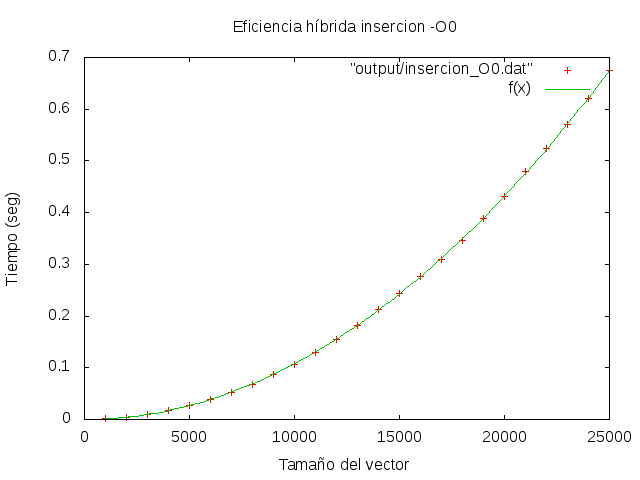
\includegraphics[width=0.6\textwidth]{../plots/insercion_O0_fit.png}}%
    \caption{Ajuste para: ordenación usando el algoritmo de inserción}%
\end{figure}

\begin{verbatim}
Final set of parameters            Asymptotic Standard Error
=======================            ==========================

a               = 1.08271e-09      +/- 6.279e-12    (0.5799%)
b               = -7.7687e-08      +/- 1.682e-07    (216.5%)
c               = 0.000123925      +/- 0.0009489    (765.7%)


\end{verbatim}


\subsection{Algoritmo de ordenación por selección}


\begin{figure}[H]%
    \centering
    \subfloat[Nube de puntos]{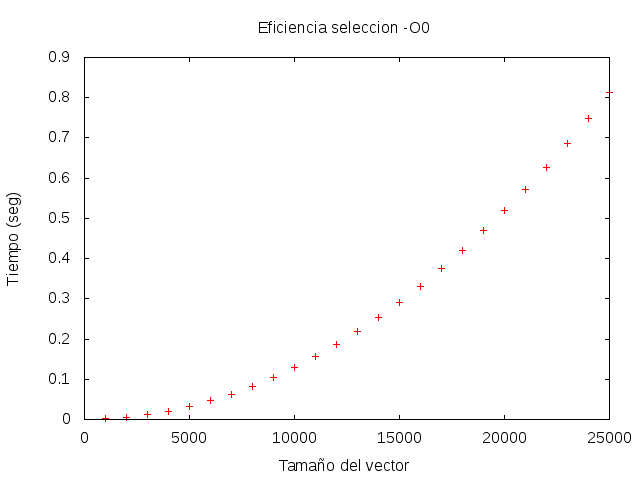
\includegraphics[width=0.5\textwidth]{../plots/seleccion_O0_points.png}}%
    \subfloat[Función continua]{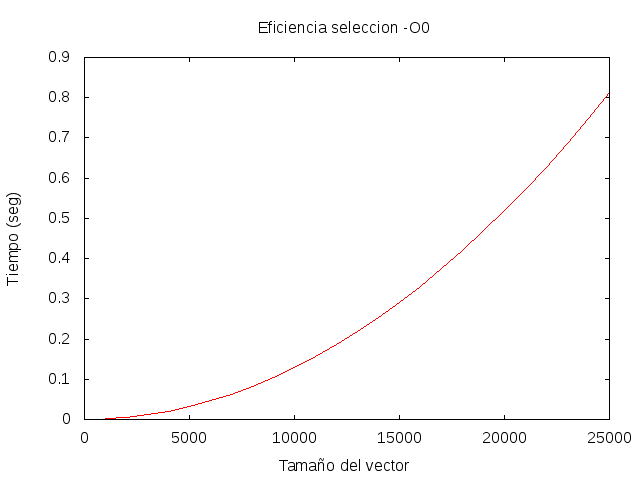
\includegraphics[width=0.5\textwidth]{../plots/seleccion_O0_lines.png}}%
    \caption{Resultados experimentales representados mediante una nube de puntos y la linea que los une}%
    \centering
    \subfloat{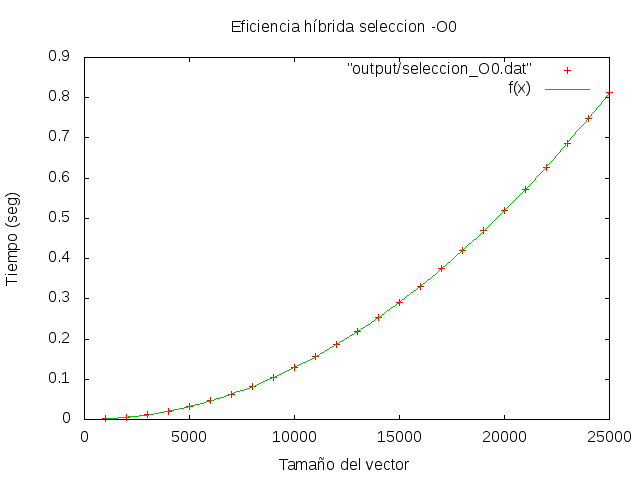
\includegraphics[width=0.6\textwidth]{../plots/seleccion_O0_fit.png}}%
    \caption{Ajuste para: ordenación usando el algoritmo de selección}%
\end{figure}

\begin{verbatim}
Final set of parameters            Asymptotic Standard Error
=======================            ==========================

a               = 1.30761e-09      +/- 1.868e-12    (0.1429%)
b               = -2.41748e-07     +/- 5.005e-08    (20.7%)
c               = 0.000572432      +/- 0.0002824    (49.33%)


\end{verbatim}


\subsection{Comparativa de los algoritmos cuadráticos de ordenación}

\subsection{Algoritmo de ordenación mergesort}

\begin{figure}[H]%
    \centering
    \subfloat[Nube de puntos]{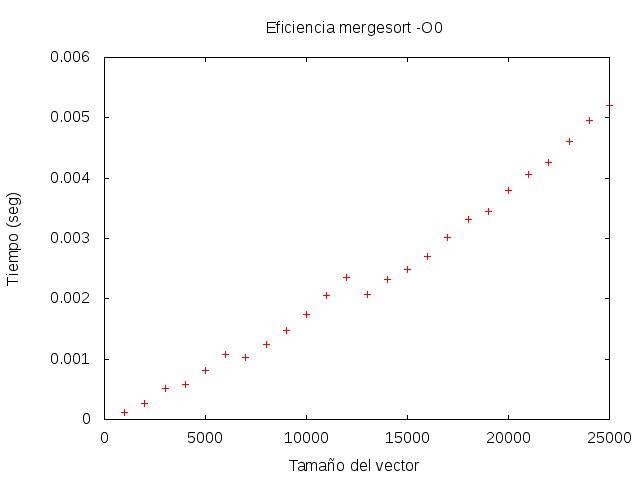
\includegraphics[width=0.5\textwidth]{../plots/mergesort_O0_points.png}}%
    \subfloat[Función continua]{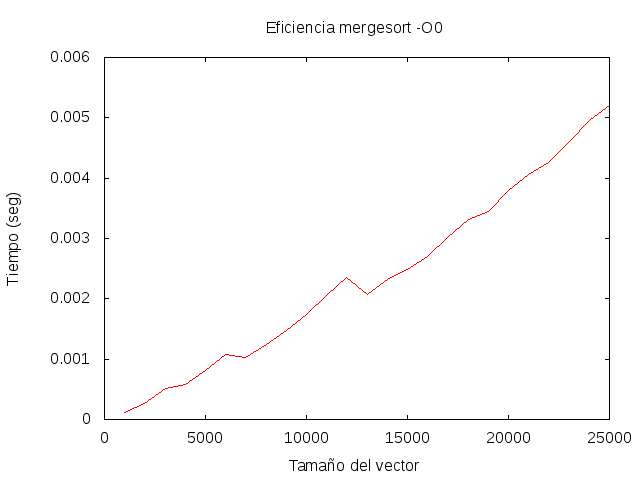
\includegraphics[width=0.5\textwidth]{../plots/mergesort_O0_lines.png}}%
    \caption{Resultados experimentales representados mediante una nube de puntos y la linea que los une}%
    \centering
    \subfloat{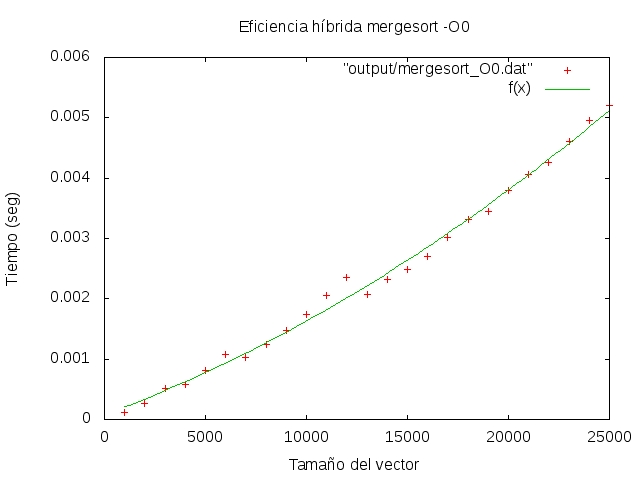
\includegraphics[width=0.6\textwidth]{../plots/mergesort_O0_fit.png}}%
    \caption{Ajuste para: ordenación usando el algoritmo mergesort}%
\end{figure}

\begin{verbatim}
Final set of parameters            Asymptotic Standard Error
=======================            ==========================

a               = 0.00162555       +/- 0.0003876    (23.85%)
b               = 1.00697          +/- 964.1        (9.575e+04%)
c               = -0.0126195       +/- 0.003794     (30.07%)


\end{verbatim}

\subsection{Algoritmo de ordenación quicksort}

\begin{figure}[H]%
    \centering
    \subfloat[Nube de puntos]{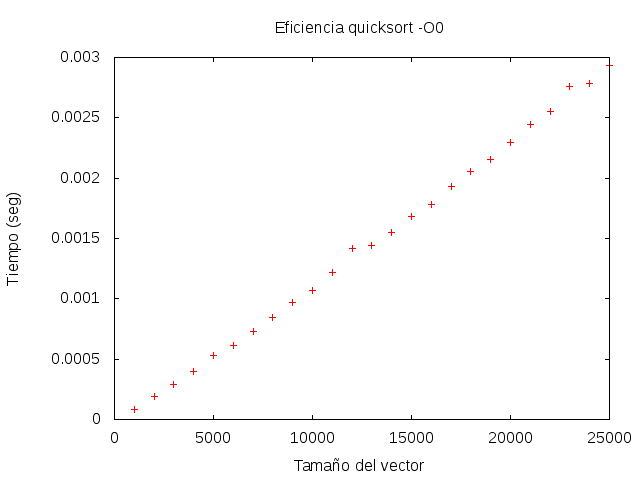
\includegraphics[width=0.5\textwidth]{../plots/quicksort_O0_points.png}}%
    \subfloat[Función continua]{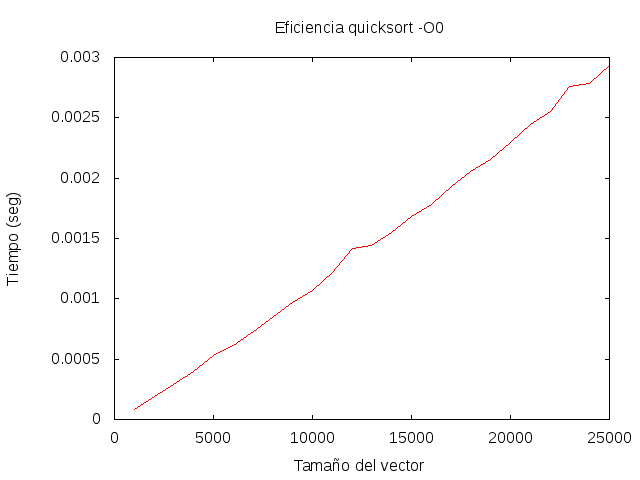
\includegraphics[width=0.5\textwidth]{../plots/quicksort_O0_lines.png}}%
    \caption{Resultados experimentales representados mediante una nube de puntos y la linea que los une}%
    \centering
    \subfloat{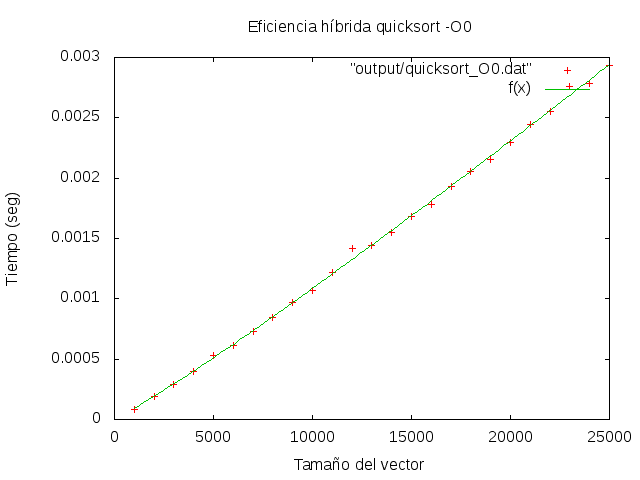
\includegraphics[width=0.6\textwidth]{../plots/quicksort_O0_fit.png}}%
    \caption{Ajuste para: ordenación usando el algoritmo quicksort}%
\end{figure}

\begin{verbatim}
Final set of parameters            Asymptotic Standard Error
=======================            ==========================

a               = 0.000967764      +/- 0.0001992    (20.58%)
b               = 1.00236          +/- 832.3        (8.303e+04%)
c               = -0.00746142      +/- 0.00195      (26.13%)


\end{verbatim}

\subsection{Algoritmo de ordenación heapsort}

\begin{figure}[H]%
    \centering
    \subfloat[Nube de puntos]{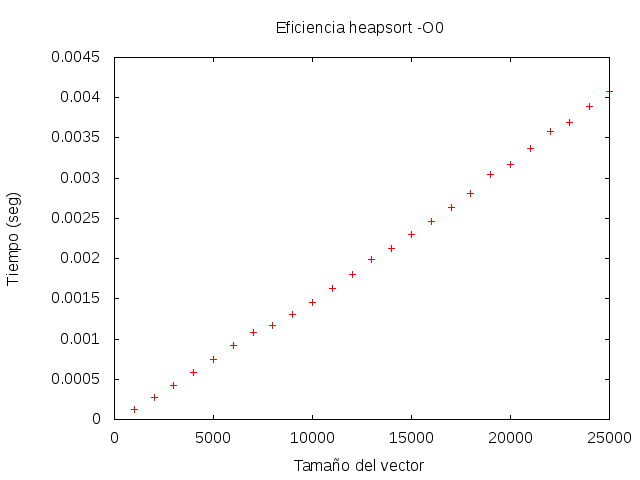
\includegraphics[width=0.5\textwidth]{../plots/heapsort_O0_points.png}}%
    \subfloat[Función continua]{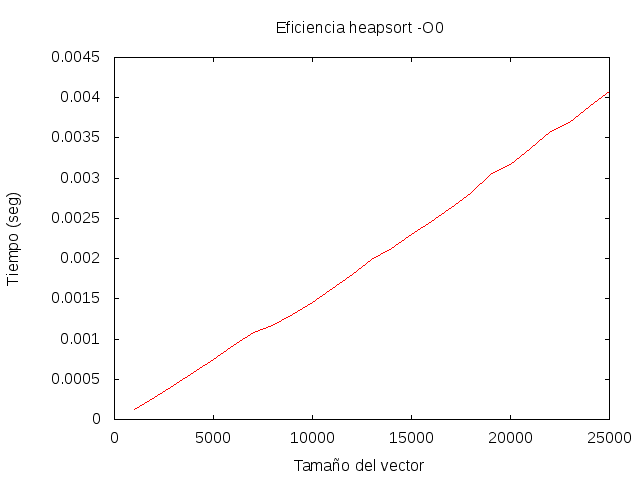
\includegraphics[width=0.5\textwidth]{../plots/heapsort_O0_lines.png}}%
    \caption{Resultados experimentales representados mediante una nube de puntos y la linea que los une}%
    \centering
    \subfloat{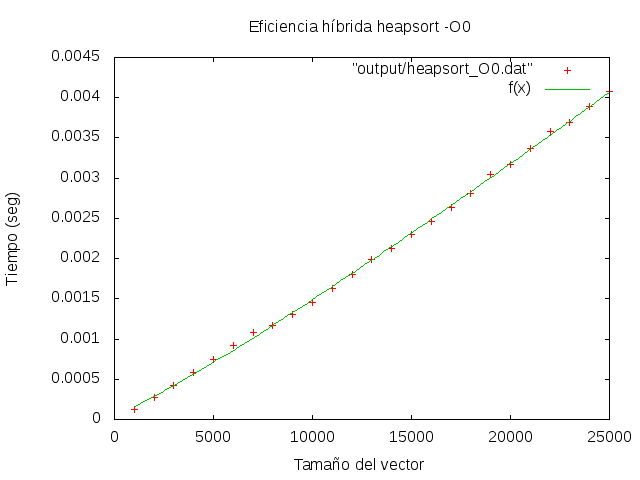
\includegraphics[width=0.6\textwidth]{../plots/heapsort_O0_fit.png}}%
    \caption{Ajuste para: ordenación usando el algoritmo heapsort}%
\end{figure}

\begin{verbatim}
Final set of parameters            Asymptotic Standard Error
=======================            ==========================

a               = 0.00132491       +/- 0.0002776    (20.95%)
b               = 1.00436          +/- 847.2        (8.436e+04%)
c               = -0.0102003       +/- 0.002718     (26.64%)


\end{verbatim}

\subsection{Algoritmo floyd}

\begin{figure}[H]%
    \centering
    \subfloat[Nube de puntos]{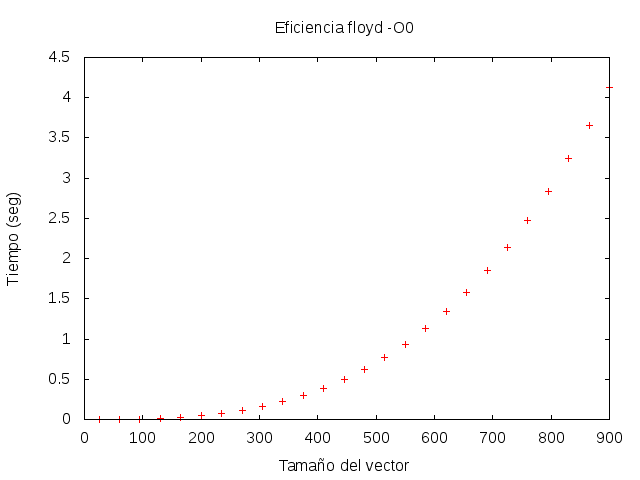
\includegraphics[width=0.5\textwidth]{../plots/floyd_O0_points.png}}%
    \subfloat[Función continua]{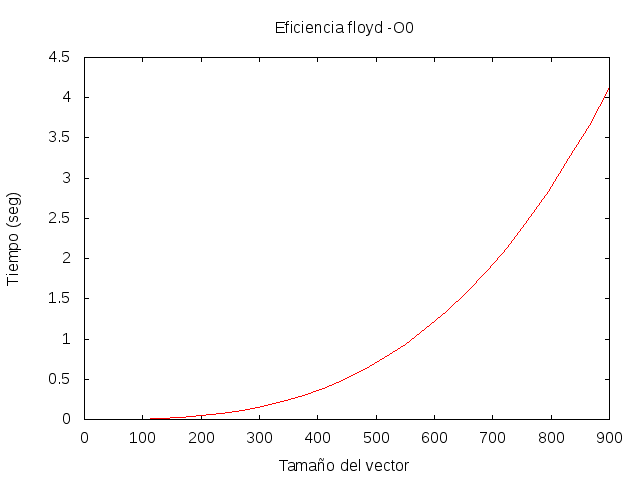
\includegraphics[width=0.5\textwidth]{../plots/floyd_O0_lines.png}}%
    \caption{Resultados experimentales representados mediante una nube de puntos y la linea que los une}%
    \centering
    \subfloat{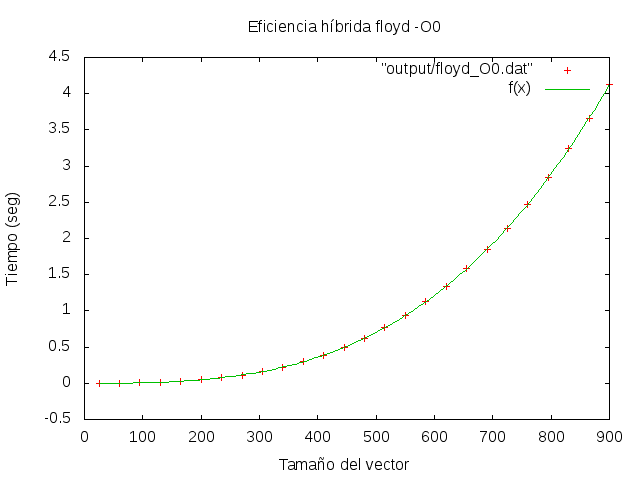
\includegraphics[width=0.6\textwidth]{../plots/floyd_O0_fit.png}}%
    \caption{Ajuste para: algoritmo para calculo de costo floyd}%
\end{figure}

\begin{verbatim}

\end{verbatim}

\subsection{Algoritmo de las torres de Hanoi}

\begin{figure}[H]%
    \centering
    \subfloat[Nube de puntos]{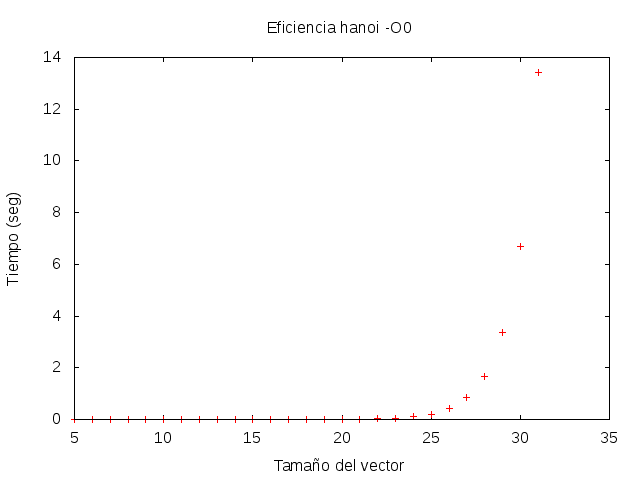
\includegraphics[width=0.5\textwidth]{../plots/hanoi_O0_points.png}}%
    \subfloat[Función continua]{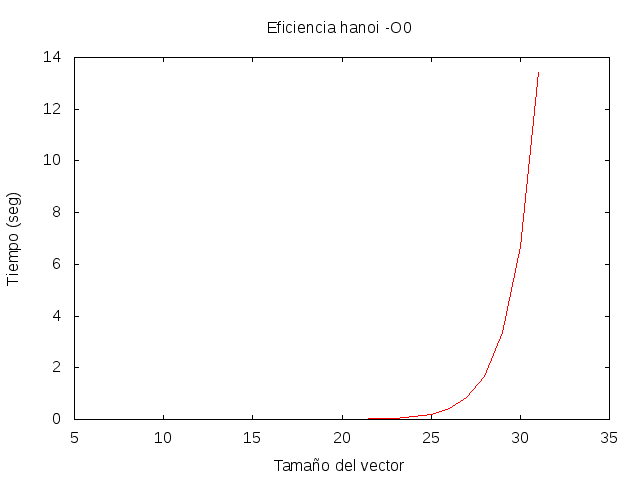
\includegraphics[width=0.5\textwidth]{../plots/hanoi_O0_lines.png}}%
    \caption{Resultados experimentales representados mediante una nube de puntos y la linea que los une}%
    \centering
    \subfloat{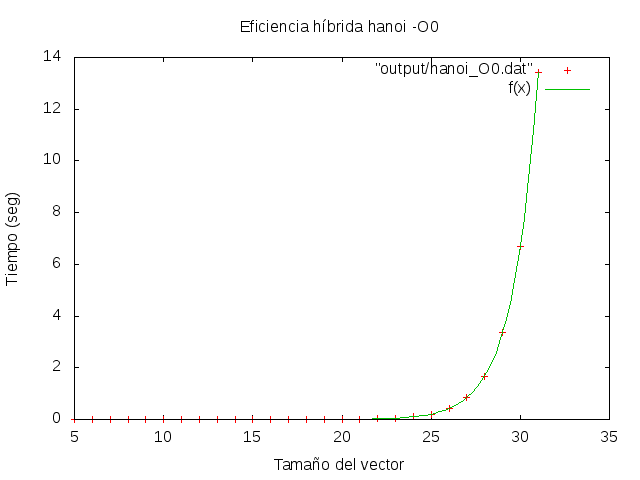
\includegraphics[width=0.6\textwidth]{../plots/hanoi_O0_fit.png}}%
    \caption{Ajuste para: calculo de los movimientos en las torres de hanoi}%
\end{figure}

\begin{verbatim}

\end{verbatim}


\section{Analisis de los resultados}

\subsection{Comparativa de los algoritmos $O(n^2)$ de ordenación}

\begin{figure}[H]
  \centering   
      \subfloat {%

        \begin{tabular}[H]{|llll|}
\hline
\textbf{Tamaño} & \textbf{Burbuja} & \textbf{Insercción} & \textbf{Selección} \\ \hline
0 & 0.004246 & 0.00112 & 0.00135595 \\ \hline
1000 & 0.008201 & 0.004292 & 0.00524505 \\ \hline
2000 & 0.019307 & 0.009728 & 0.011705 \\ \hline
3000 & 0.034225 & 0.017294 & 0.020711 \\ \hline
4000 & 0.056845 & 0.026957 & 0.03227 \\ \hline
5000 & 0.088076 & 0.038868 & 0.046363 \\ \hline
6000 & 0.120856 & 0.052248 & 0.062962 \\ \hline
7000 & 0.161862 & 0.068156 & 0.082298 \\ \hline
8000 & 0.210286 & 0.086587 & 0.104299 \\ \hline
9000 & 0.264146 & 0.107304 & 0.128745 \\ \hline
10000 & 0.323677 & 0.130252 & 0.156038 \\ \hline
11000 & 0.394902 & 0.15566 & 0.185971 \\ \hline
12000 & 0.463354 & 0.182503 & 0.218305 \\ \hline
13000 & 0.541129 & 0.212983 & 0.253628 \\ \hline
14000 & 0.628463 & 0.243724 & 0.291057 \\ \hline
15000 & 0.718559 & 0.2767 & 0.331193 \\ \hline
16000 & 0.814468 & 0.309732 & 0.374365 \\ \hline
17000 & 0.919391 & 0.346489 & 0.419854 \\ \hline
18000 & 1.03422 & 0.387793 & 0.469411 \\ \hline
19000 & 1.14783 & 0.432006 & 0.518467 \\ \hline
20000 & 1.27545 & 0.479765 & 0.571629 \\ \hline
21000 & 1.39817 & 0.524347 & 0.62718 \\ \hline
22000 & 1.53151 & 0.569582 & 0.68739 \\ \hline
23000 & 1.67702 & 0.620089 & 0.747746 \\ \hline
24000 & 1.81403 & 0.675667 & 0.81211 \\ \hline

\end{tabular}
        
      }
      
      \subfloat{%
        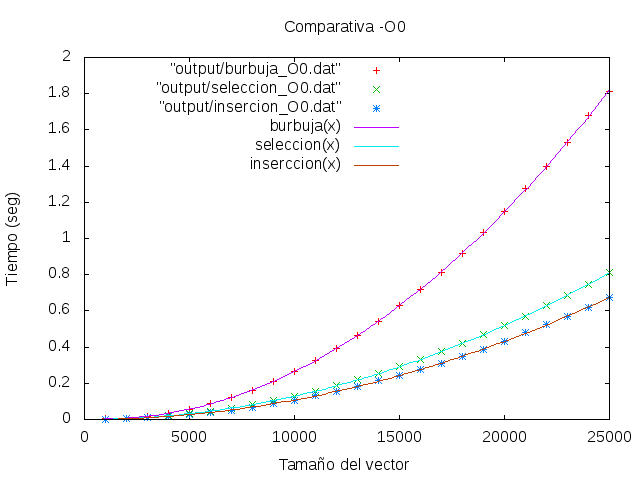
\includegraphics[clip,width=0.7\columnwidth]{../plots/cuadraticas_O0.png}%
      }



\caption{Comaparación entre los distintos algoritmos de ordenación cuadráticos}
\end{figure}


\subsection{Comparativa de los algoritmos $nlog(n)$ de ordenación}

\begin{figure}[H]
  \centering   
      \subfloat {%

        \begin{tabular}[H]{|llll|}
\hline
\textbf{Tamaño} & \textbf{Mergesort} & \textbf{Quicksort} & \textbf{Heapesort} \\ \hline
0 & 0.000117755 & 8.7e-05 & 0.000124 \\ \hline
1000 & 0.000265505 & 0.000187 & 0.000268 \\ \hline
2000 & 0.000509884 & 0.000294 & 0.000422 \\ \hline
3000 & 0.000580912 & 0.000394 & 0.000585 \\ \hline
4000 & 0.000807877 & 0.000534 & 0.000748 \\ \hline
5000 & 0.00107341 & 0.000616 & 0.00092 \\ \hline
6000 & 0.00103389 & 0.000727 & 0.001085 \\ \hline
7000 & 0.00124508 & 0.000843 & 0.001164 \\ \hline
8000 & 0.00147816 & 0.00097 & 0.001303 \\ \hline
9000 & 0.00174622 & 0.001065 & 0.00146 \\ \hline
10000 & 0.002063 & 0.001219 & 0.001627 \\ \hline
11000 & 0.002352 & 0.001415 & 0.001808 \\ \hline
12000 & 0.002076 & 0.001446 & 0.001986 \\ \hline
13000 & 0.002313 & 0.001549 & 0.00212 \\ \hline
14000 & 0.002485 & 0.001683 & 0.002294 \\ \hline
15000 & 0.002708 & 0.001781 & 0.002464 \\ \hline
16000 & 0.003018 & 0.001935 & 0.002641 \\ \hline
17000 & 0.00331 & 0.002054 & 0.002815 \\ \hline
18000 & 0.003453 & 0.002157 & 0.00305 \\ \hline
19000 & 0.00379 & 0.002295 & 0.003175 \\ \hline
20000 & 0.004064 & 0.002443 & 0.003364 \\ \hline
21000 & 0.004262 & 0.002554 & 0.003576 \\ \hline
22000 & 0.004612 & 0.002758 & 0.003686 \\ \hline
23000 & 0.004959 & 0.002788 & 0.003889 \\ \hline
24000 & 0.005205 & 0.002935 & 0.004078 \\ \hline

\end{tabular}
        
      }
      
      \subfloat{%
        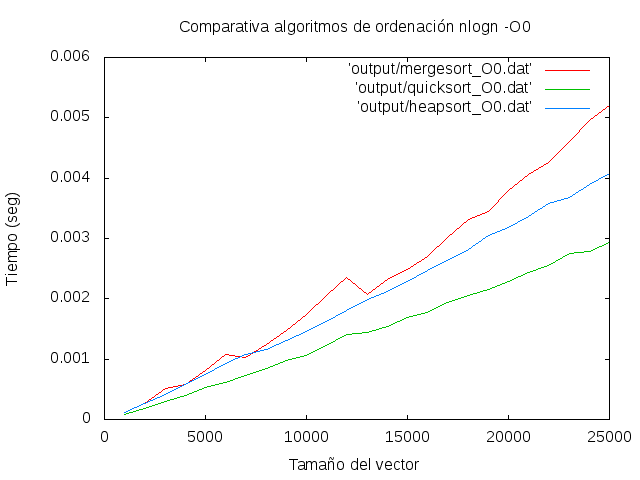
\includegraphics[clip,width=0.7\columnwidth]{../plots/logaritmicos_O0.png}%
      }
      \caption{Comaparación entre los distintos algoritmos de ordenación $nlogn$}
\end{figure}

\subsection{Comparativa de los algoritmos de ordenación}

\begin{figure}[H]
  \centering   
      \subfloat {%
        \begin{tabular}[H]{|lllllll|}
\hline
\textbf{Tamaño} & \textbf{Burbuja} & \textbf{Inserción} & \textbf{Selección} & \textbf{Mergesort} & \textbf{Quicksort} & \textbf{Heapesort} \\ \hline
0 & 0.004246 & 0.00112 & 0.00135595 & 0.000117755 & 8.7e-05 & 0.000124 \\ \hline
1000 & 0.008201 & 0.004292 & 0.00524505 & 0.000265505 & 0.000187 & 0.000268 \\ \hline
2000 & 0.019307 & 0.009728 & 0.011705 & 0.000509884 & 0.000294 & 0.000422 \\ \hline
3000 & 0.034225 & 0.017294 & 0.020711 & 0.000580912 & 0.000394 & 0.000585 \\ \hline
4000 & 0.056845 & 0.026957 & 0.03227 & 0.000807877 & 0.000534 & 0.000748 \\ \hline
5000 & 0.088076 & 0.038868 & 0.046363 & 0.00107341 & 0.000616 & 0.00092 \\ \hline
6000 & 0.120856 & 0.052248 & 0.062962 & 0.00103389 & 0.000727 & 0.001085 \\ \hline
7000 & 0.161862 & 0.068156 & 0.082298 & 0.00124508 & 0.000843 & 0.001164 \\ \hline
8000 & 0.210286 & 0.086587 & 0.104299 & 0.00147816 & 0.00097 & 0.001303 \\ \hline
9000 & 0.264146 & 0.107304 & 0.128745 & 0.00174622 & 0.001065 & 0.00146 \\ \hline
10000 & 0.323677 & 0.130252 & 0.156038 & 0.002063 & 0.001219 & 0.001627 \\ \hline
11000 & 0.394902 & 0.15566 & 0.185971 & 0.002352 & 0.001415 & 0.001808 \\ \hline
12000 & 0.463354 & 0.182503 & 0.218305 & 0.002076 & 0.001446 & 0.001986 \\ \hline
13000 & 0.541129 & 0.212983 & 0.253628 & 0.002313 & 0.001549 & 0.00212 \\ \hline
14000 & 0.628463 & 0.243724 & 0.291057 & 0.002485 & 0.001683 & 0.002294 \\ \hline
15000 & 0.718559 & 0.2767 & 0.331193 & 0.002708 & 0.001781 & 0.002464 \\ \hline
16000 & 0.814468 & 0.309732 & 0.374365 & 0.003018 & 0.001935 & 0.002641 \\ \hline
17000 & 0.919391 & 0.346489 & 0.419854 & 0.00331 & 0.002054 & 0.002815 \\ \hline
18000 & 1.03422 & 0.387793 & 0.469411 & 0.003453 & 0.002157 & 0.00305 \\ \hline
19000 & 1.14783 & 0.432006 & 0.518467 & 0.00379 & 0.002295 & 0.003175 \\ \hline
20000 & 1.27545 & 0.479765 & 0.571629 & 0.004064 & 0.002443 & 0.003364 \\ \hline
21000 & 1.39817 & 0.524347 & 0.62718 & 0.004262 & 0.002554 & 0.003576 \\ \hline
22000 & 1.53151 & 0.569582 & 0.68739 & 0.004612 & 0.002758 & 0.003686 \\ \hline
23000 & 1.67702 & 0.620089 & 0.747746 & 0.004959 & 0.002788 & 0.003889 \\ \hline
24000 & 1.81403 & 0.675667 & 0.81211 & 0.005205 & 0.002935 & 0.004078 \\ \hline

\end{tabular}
      }
      
      \subfloat{%
        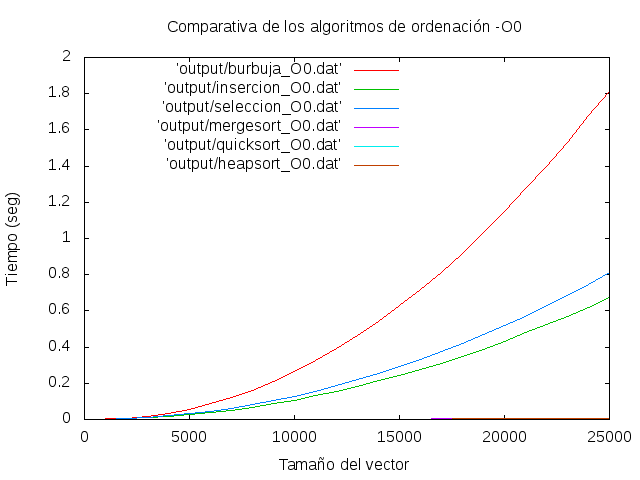
\includegraphics[clip,width=0.7\columnwidth]{../plots/todos_ordenacion_O0.png}%
      }
      \caption{Comaparación entre los distintos algoritmos de ordenación $nlogn$}
\end{figure}

De los resultados obtenidos podemos ver de forma clara como el
algoritmo de burbuja es el que desempeña la tarea de forma
considerablemente más lenta.

Entre los algoritmos de selección e insercción no encontramos mucha
diferencia aunque son notoriamente más eficientes que el de burbuja.

Finalmente los algoritmos de orden $O(n\cdot log(n))$ son mucho más
eficientes que el resto aunque podemos observar como el algoritmo
quicksort ha sido el que ha obtenido mejores resultados pese a ser del
mismo orden de eficiencia.

En el algoritmo de hanoi podemos observar como al ser $O(2^n)$ el
tiempo que tarda en ejecutarse crece rapidamente a partir de un punto
lo cual nos permite realizar únicamente pocas iteraciones.

\end{document}